\documentclass{beamer}

\usetheme{Rochester}

\beamertemplatenavigationsymbolsempty
\usepackage[english]{babel}
\usepackage{xcolor}
\usecolortheme{beaver}

%\usefonttheme{serif}
%\usepackage{palatino}

\title{ ~ \\ ~ \\ {\huge{AdaProp}} \\ ~ \\ 
    {\large Adaptive Propositionalisation of Multi-Instance Data Towards Image Classification} \\ ~ }
\subtitle{}

\author{~ \\ ~\\ Siva~Manoharan \\~\\ Supervisor: Dr.~Eibe~Frank}

\date{}

% Customizing colours:
\definecolor{primaryfg}{RGB}{170, 0, 0}
\setbeamercolor*{item}{fg=darkred!60!black}
%\setbeamercolor{itemize subitem}{fg=primaryfg}
%\setbeamercolor{itemize subsubitem}{fg=primaryfg}
%\setbeamercolor{enumerate item}{fg=primaryfg}
%\setbeamercolor{enumerate subitem}{fg=primaryfg}
%\setbeamercolor{enumerate subsubitem}{fg=primaryfg}

\setbeamercolor{title}{fg=darkred!80!black} 
\setbeamercolor{background canvas}{bg=white!97!black}
\setbeamercolor{headline}{bg=white!90!black}
\setbeamertemplate{headline}[text line]{%
  %\begin{beamercolorbox}[wd=\paperwidth,ht=2cm, dp=.2cm, leftskip=.5cm,rightskip=.3cm]{headline}%
  \begin{beamercolorbox}[wd=\paperwidth,ht=2cm]{headline}%
  \end{beamercolorbox}%
}


% If you have a file called "university-logo-filename.xxx", where xxx
% is a graphic format that can be processed by latex or pdflatex,
% resp., then you can add a logo as follows:

% \pgfdeclareimage[height=0.5cm]{university-logo}{university-logo-filename}
% \logo{\pgfuseimage{university-logo}}



% Delete this, if you do not want the table of contents to pop up at
% the beginning of each subsection:
%\AtBeginSubsection[]
%{
%  \begin{frame}<beamer>{Outline}
%    \tableofcontents[currentsection,currentsubsection]
%  \end{frame}
%}


% If you wish to uncover everything in a step-wise fashion, uncomment
% the following command: 

%\beamerdefaultoverlayspecification{<+->}


\begin{document}
{
%\setbeamertemplate{headline}{}
\makeatletter % to change template
    \setbeamercolor{headline}{bg=white!97!black}
    %\setbeamertemplate{headline}[default] % not mandatory, but I though it was better to set it blank
    \def\beamer@entrycode{\vspace*{-\headheight}} % here is the part we are interested in :)
\makeatother

\begin{frame}
  \titlepage
\end{frame}
}

\begin{frame}{Image Classification}
\vspace{-0.5cm}
    \begin{itemize}
        \item Does the Image contain a specific object?
    \end{itemize}
\vspace{-0.5cm}
  \begin{columns}[T]
    \begin{column}{.5\textwidth}
    \begin{center} 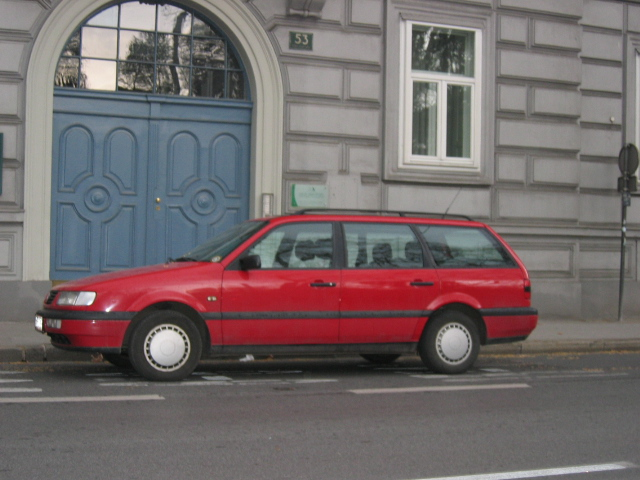
\includegraphics[scale=0.25]{img/cars1} \\~\\ {\Large Car} \end{center}
    \end{column}
    \begin{column}{.5\textwidth}
    \begin{center} 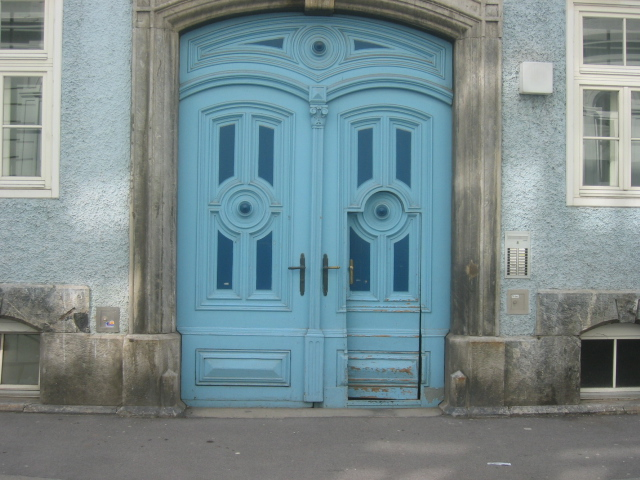
\includegraphics[scale=0.25]{img/none1} \\~\\ {\Large None}  \end{center}
    \end{column}
  \end{columns}
  
\end{frame}

\begin{frame}{Image Classification}
\vspace{-0.5cm}
    \begin{itemize}
        \item Not easy in practice (for computers)
    \end{itemize}
\vspace{-0.5cm}
  \begin{columns}[T]
    \begin{column}{.5\textwidth}
    \begin{center} 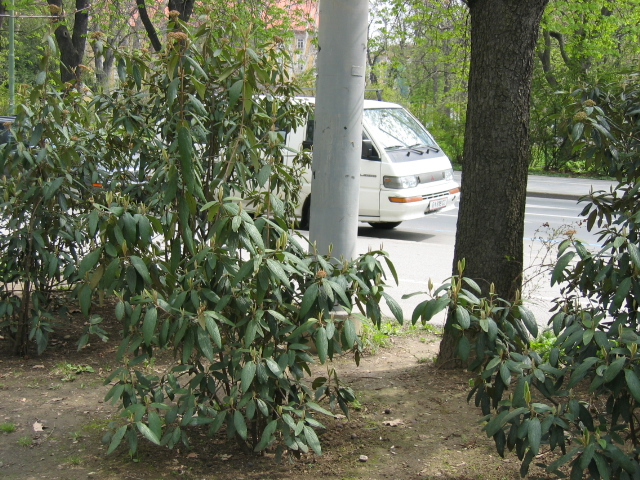
\includegraphics[scale=0.25]{img/cars2} \\~\\ {\Large Partial Occlusion} \end{center}
    \end{column}
    \begin{column}{.5\textwidth}
    \begin{center} 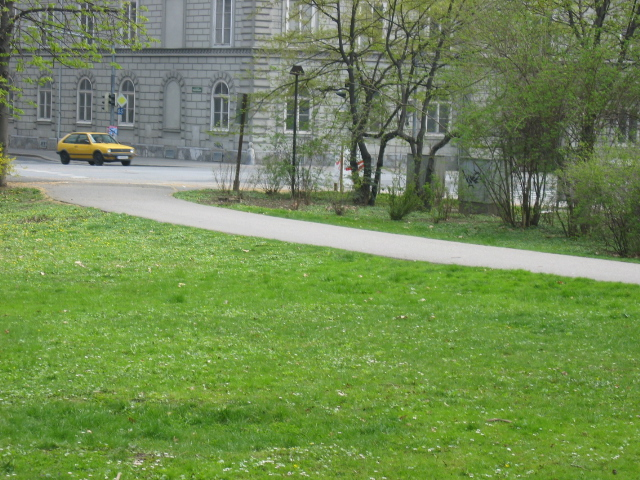
\includegraphics[scale=0.25]{img/cars3} \\~\\ {\Large Not in Foreground}  \end{center}
    \end{column}
  \end{columns}
  
\end{frame}


\begin{frame}{Multi-Instance Learning}

    \begin{itemize}
        \item A good fit for Image Classification \\ ~
        \item Also used for Text and Chemical datasets \\ ~
        \item Key: Bags of Instances
    \end{itemize}
    % TODO: show splitting? (not enough time)
\end{frame}

\begin{frame}{Propositionalisation}

    \begin{itemize}
        \item \dots \\ ~
        \item \dots \\ ~
        \item \dots
    \end{itemize}
    % TODO: Lots more algorithms in stardard mi
\end{frame}

\begin{frame}{AdaProp: Adaptive Propositionalisation}

    \begin{itemize}
        \item \dots \\ ~
        \item \dots \\ ~
        \item \dots
    \end{itemize}
    % TODO: Needs diagram
    % Mention WEKA? Screenshot of params?
\end{frame}

\begin{frame}{Results: Impact of \dots}

    \begin{itemize}
        \item \dots \\ ~
        \item \dots \\ ~
        \item \dots
    \end{itemize}
    % TODO: 
\end{frame}

\begin{frame}{Results: \dots vs \dots}

    \begin{itemize}
        \item \dots \\ ~
        \item \dots \\ ~
        \item \dots
    \end{itemize}
    % TODO: 
\end{frame}

\begin{frame}{Summary}

  % Keep the summary *very short*.
  \begin{itemize}
  \item
    The \alert{first main message} of your talk in one or two lines. \\ ~
  \item
    The \alert{second main message} of your talk in one or two lines. \\ ~
  \item
    To do in the future \alert{third message}
  \end{itemize}
  
\end{frame}



\end{document}


